\section{Evaluation protocol}
\label{sec:protocol}

\begin{figure}[htbp]
\centering
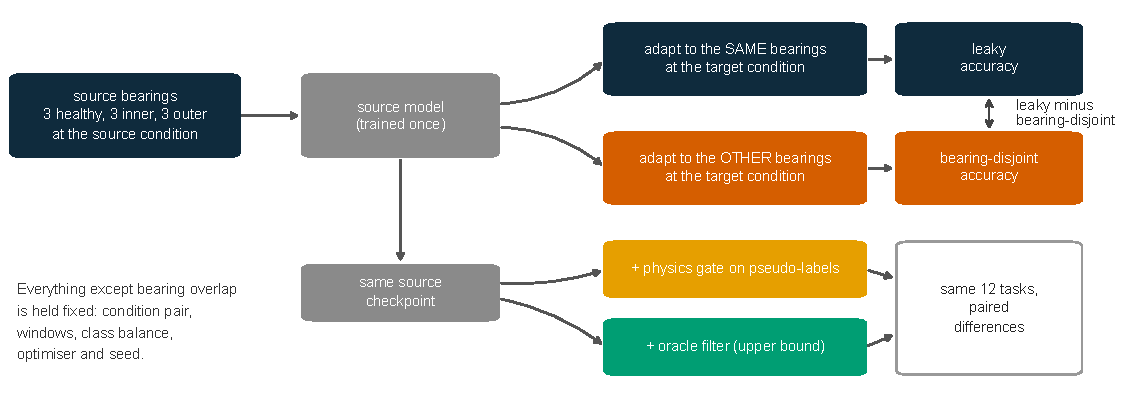
\includegraphics[width=\linewidth]{figures/fig1_design.pdf}
\caption{The paired design. One source model is trained on the source bearings at the source condition and then adapted
twice: to the \emph{same} bearings at the target condition (leaky) and to the complementary bearings at the same target
condition (clean). Both targets share the operating condition, the window contract and the class balance, so their
difference isolates bearing overlap. Gated and oracle arms reuse the same source checkpoint.}
\label{fig:design}
\end{figure}

\subsection{The paired leaky/clean design}

A source bearing set of 3 healthy, 3 outer-race and 3 inner-race specimens is trained at one operating condition. The
resulting source model is then adapted, without target labels, to two different targets at the same target condition
(Fig.~\ref{fig:design}): the \emph{leaky} target, made of the same physical bearings, and the \emph{clean} target, made of
the complementary bearings. Every other factor is held fixed --- operating condition, window length, number of windows per
class, class balance, optimiser, schedule and seed --- so the leaky--clean difference, written
$\Delta_{\mathrm{leak}}$, is attributable to bearing overlap alone. With three conditions there are six ordered condition
pairs, hence six tasks per split and per direction.

Windows are 2048 samples with 2000 windows per class, balanced across the classes and spread evenly over that class's
bearings and recordings; no window crosses a recording boundary. This window contract is inherited from the released SDALR
configuration so that the reproduction of Section~\ref{sec:res-repro} is faithful.

\subsection{Splits}

\begin{table}[htbp]
\centering
\caption{Source bearing sets on Paderborn.}
\label{tab:splits}
\small
\setlength{\tabcolsep}{4pt}
\begin{tabular}{llll}
\toprule
Split & Healthy & Outer race & Inner race \\
\midrule
fold A & K001, K002, K003 & KA04, KA15, KA16 & KI04, KI14, KI16 \\
fold B & K004, K005, K006 & KA22, KA30 & KI17, KI18, KI21 \\
\midrule
S00 & K001, K003, K004 & KA16, KA22, KA30 & KI04, KI16, KI18 \\
S01 & K002, K004, K006 & KA15, KA22, KA30 & KI04, KI17, KI21 \\
S02 & K002, K003, K005 & KA15, KA16, KA30 & KI16, KI17, KI21 \\
S03 & K002, K003, K004 & KA04, KA16, KA22 & KI16, KI18, KI21 \\
S04 & K001, K002, K006 & KA15, KA16, KA30 & KI04, KI14, KI18 \\
S05 & K003, K005, K006 & KA04, KA16, KA30 & KI04, KI17, KI21 \\
S06 & K002, K003, K006 & KA16, KA22, KA30 & KI04, KI17, KI18 \\
S07 & K003, K005, K006 & KA04, KA16, KA22 & KI04, KI14, KI16 \\
S08 & K001, K002, K006 & KA15, KA22, KA30 & KI04, KI16, KI21 \\
S09 & K002, K003, K005 & KA04, KA15, KA16 & KI16, KI17, KI21 \\
\bottomrule
\end{tabular}
\begin{minipage}{\linewidth}\vspace{2pt}\footnotesize The clean target of each row is the complement within the real-damage pool (6 healthy, 5 outer-race, 6 inner-race); the leaky target is the same bearings at the target operating condition. S00--S09 were drawn uniformly without replacement from the 4{,}000 possible 3/3/3 draws with a seed fixed before any run.\end{minipage}
\end{table}


Two families of splits are used on Paderborn (Table~\ref{tab:splits}). The two \emph{mechanical folds} follow a fixed rule
--- within each (damage origin, fault type) group, sort bearing codes lexicographically and assign the first half to fold A
--- and are run in both directions, which gives 12 paired tasks. Because two folds are two draws out of the 4000 possible
3/3/3 source sets, we additionally drew ten source sets uniformly without replacement from those 4000, excluding fold A,
with the random seed and the draw list fixed in version control before any of these runs. The \emph{split} is the
statistical unit for the ten-split analyses; tasks are the unit within a fold. On HUST the same construction uses bearing
types: the source is three of the five types and the clean target is the other two, for six pre-registered splits.

\subsection{Adaptation variants}

SDALR is run from its released code with two checkpoint policies. \texttt{as\_released} keeps the released selection rule,
which compares target accuracy against its initial value and therefore consults target labels; \texttt{final\_checkpoint}
takes the last iterate and touches no target label at any point. All headline numbers use \texttt{final\_checkpoint};
\texttt{as\_released} is reported once, in Section~\ref{sec:res-collapse}, to quantify what target-label checkpoint
selection contributes. SHOT is implemented on the same backbone, data pipeline and schedule, with a frozen classifier head,
information-maximisation loss and centroid pseudo-labels recomputed each epoch, and is evaluated at the last iterate.

\subsection{Gating, pairing and the oracle ceiling}

A gate returns one verdict per \emph{recording}, in $\{\text{silent},\text{inner race},\text{outer race}\}$, which every
window of that recording inherits; silence is not a healthy verdict. Inside the adaptation loop the verdict acts on the
method's own pseudo-label step: where the gate speaks, a pseudo-label is kept only if it agrees with the verdict, and is
otherwise withheld from the supervised term; where the gate is silent, the method is unchanged. The \emph{oracle filter}
replaces the verdict by the true label, keeping only correct pseudo-labels, and therefore measures what a perfect
pseudo-label filter could achieve within the same adaptation procedure.

All arms of a comparison --- ungated, each gate, oracle --- run in the same job from the same source checkpoint with the
same seed, so the comparison is paired. We verify this from the logs rather than asserting it: the pre-update accuracy on
the target, recorded before any adaptation step, is identical across arms in every task. Effects are therefore reported as
distributions of per-task differences, not as differences of means.

The collapse is decomposed as
\begin{equation}
\underbrace{a_{\mathrm{leaky}}-a_{\mathrm{clean}}}_{\text{total}}
=\underbrace{\left(a_{\mathrm{oracle}}-a_{\mathrm{clean}}\right)}_{\text{filter-recoverable}}
+\underbrace{\left(a_{\mathrm{leaky}}-a_{\mathrm{oracle}}\right)}_{\text{not filter-recoverable}},
\label{eq:decomp}
\end{equation}
where $a$ denotes accuracy under the arm named in the subscript. The second term is what no pseudo-label filter can reach,
because it remains when every kept pseudo-label is correct.

\subsection{Statistics and pre-registration}

Effects are paired differences. Within a fold, however, the twelve tasks share source checkpoints and bearing sets, so
treating them as independent units overstates the evidence. We therefore report every primary effect three ways: the
task-level one-sided Wilcoxon signed-rank test (descriptive only), a bootstrap that resamples whole clusters, and an exact
permutation test that flips the sign of entire clusters. The cluster is the source fold for the fold experiments and the
split elsewhere. With two folds an exact cluster-level test cannot fall below $p = 0.25$, so \emph{the fold experiments are
descriptive and the ten random splits carry the inference}. Across the family of primary tests, cluster-level $p$-values are
adjusted by the Benjamini--Hochberg procedure \cite{benjamini2001}; the collapse and the gate gain over ten splits survive
adjustment ($p_{\mathrm{BH}} = 0.005$ and $0.007$). Intervals on record-level rates use a bearing-cluster bootstrap, because
recordings of one bearing are not independent.

Arms are never crossed between jobs. Running one configuration twice gives slightly different numbers (up to 1.6~pp on a
fold mean, from non-deterministic GPU reductions), so each comparison uses the arms produced inside a single job: the
leaky--clean contrast comes from the fold job, and the gated and oracle arms are compared against the ungated arm of the
gating job. Both values are reported where they differ.

Every hypothesis, decision rule, arm and budget in this paper was written into a versioned protocol before the
corresponding runs, including the gate operating points used in Section~\ref{sec:res-gating} ($z = 10$ for the envelope
rule, $\alpha = 0.05$ for the comb tests), which were fixed before any gate was evaluated; the operating-curve sweep reported later in
that section is a sensitivity analysis reported afterwards, not a selection mechanism. Each numbered change is listed
in Supplementary~S1 with what was pre-registered, what changed and why. Two consequences are visible in the paper: results
that failed their pre-registered rule are reported as such (Section~\ref{sec:res-slip}), and one planned remedy experiment
was cut for budget before any of its outcomes were seen, so no result from it appears here. Every reported number carries a
run identifier in an append-only ledger with the retained artifact and its checksum (Supplementary~S4).
